\chapter{Higgs decaying to two photons}

The Higgs to two photon channel is one of the most promising decays in the search for the SM higgs
at the LHC. Despite having a relatively small branching ratio, the decay $\Hgg$ 
provides a very clean, fully reconstructable final-state topology, making it 
one of the most sensitive channels at low mass.
The dominant source of background is from real, prompt diphoton events from QCD 
processes, $pp\rightarrow\gamma\gamma$.
In addition, there is a contribution from $pp\rightarrow\gamma+jet$ and $pp\rightarrow jet+jet$
in which jets are mis-identified as photons.
This chapter describes a search for a Higgs boson decaying to two photons
which was performed on the full 2011 dataset 
corresponding to \clumi of proton-proton collisions recorded at CMS at a center of mass energy of 7 TeV.

\section{Data samples}
\label{sec:datasamples}

The dataset used for this analysis is the combination of the 2011A and 2011B 
proton-proton collision runs.
The selection for the dataset used for this analysis is based around dedicated diphoton triggers
which select events online which satistfy one of two sets of criteria.
The first set requires two HLT photon candidates, one with $\pt>26$ GeV and the other with 
$\pt>18$ GeV, which are well isolated in the calorimeter. The second has a lower threshold on
the first photon, $\pt>22$ GeV but requires that both photons have localised showers in the ECAL 
($\rnine>0.8$ in 2011A and $\rnine>0.9$ in 2011B). 
Additionally, the invariant mass of the two trigger objects are required to have an 
invariant mass greater than 60 (70)GeV in the 2011A(B) datasets.
Events which would pass the full offline selection but failed to trigger at the HLT lead to an inefficiency, 
reducing the number of signal events with respect to that expected from an integrted luminosity of \clumi.
However, the tresholds applied offline are choson to be much tighter than those of the trigger;
the trigger efficiency is $>$99\% with respect to the analysis selection. 

Signal Monte Carlo (MC) events are generated for a Higgs decaying to two photons via the four main 
production processes, gluon-gluon fusion, vector boson fusion and assosiated $W/Z$ and $\ttbar$ production.
The gluon-gluon fusion (ggH) and vector boson fusion (qqH) were generated with \texttt{POWHEG} with 
next-to leading order (NLO) contributions whereas
the two associated production processes were generated to leading order (LO) only.
The $\pt$ spectrum of the Higgs ($\pt^{H}$) from gluon-gluon fusion was calculated at
next-to-next-to leading plus next-to leading log resummed order (NNLO+NLL) using the \texttt{HqT} program.
The production cross-sections and branching ratios are taken from the LHC Cross-section Working Group.

MC for background processes were generated at LO using \texttt{POWHEG} intefaced with \texttt{PYTHIA}.
The QCD dijet and $\gamma+jet$ samples are filtered by requiring the generated photons, electrons and neutral
mesons with $\pt>15$ GeV have at most one charged particle in a cone, $\Delta R<0.2$, to increase the 
production efficiency with respect to the tracker isolation requirements of the full selection.
The background samples considered for this analysis are summarized in Table~\ref{tab:backgroundmc}.
A full simulation of the CMS detector is provided in \texttt{GEANT4} which is used for all signal
and background MC samples.

\begin{table}
\begin{center}
\begin{tabular}{|l r|c|c|}
\hline
\textbf{Process}  & &  \textbf{Cross-section} ($pb$) & \textbf{Luminosity} ($pb^{-1}$)\\
\hline
\hline
DiPhotonJets & & 154.7 & 7400 \\
\hline
DiPhoton Box & $\hat{\pt}~25-250$ & 12.37 & 41900 \\
\hline 
QCD Dijet    & $\hat{\pt}~30-40$      & 10870 & 560 \\
	     & $\hat{\pt}~40-\infty$  & 43571 & 920 \\
\hline 
Gamma+Jet    & $\hat{\pt}~20-\infty$  & 493.44& 2400 \\
\hline 
DrellYan+Jets to $ll$  & $\hat{\pt}~50-\infty$  & 2475& 14000 \\
\hline
\end{tabular}
\caption{Background MC used throughput the analysis with production cross-sections and 
corresponding equivalent integrated luminsity.}
\label{tab:backgroundmc}
\end{center}
\end{table}


\section{Object Reconstruction and Identification}
\label{sec:objectrecoandid}

The reconstruction of all objects used in this analysis, in both data and MC
is based on the standardized CMS reconstruction software \texttt{\cmssw}. 
Additional sensitivity can be gained by refining the object selection and reconstruction specifically
to the search for $\Hgg$.


\subsection{Boosted Decision Trees}
General introduction about BDT's and what they do.
\label{sec:boosteddecisiontrees}


\subsection{Supercluster Energy Correction}
\label{superclusterenergyreconstruction}

As the natural width of Higgs boson is around 100 MeV, the width of a reconstructed mass peak from 
a $\Hgg$ decay is driven by the experimental energy resolution of the photons.
This resolution can be improved dramatically by correcting the raw energy of the supercluster 
on a per-photon level. These corrections are derived using a multivariate technique 
in which a regression BDT is trained on prompt photons in the gamma+jet MC sample using the 
ratio of the generated photon energy to the raw energy of the reconstructed supercluster.
As this ratio can vary across different regions of the detector, the input varibles include both the 
$\eta$ and $\phi$ positions of the supercluster. In addition, several variables are included which 
describe the shower shape: $\rnine$, the energy weighted widths in $\eta$ and $\phi$ of the supercluster,
the energy weighted crystal width ($\sigieie$) and the ratio of hadronic energy behind the supercluster
to the energy of the supercluster itself ($\hoe$). In the endcap, there is additional information 
available from the pre-shower. The ratio of the energy in the pre-shower to the raw supercluster energy
is included for superclusters in the ECAL endcap. Figure~\ref{fig:mcregrcomparisons} shows the improvement
in resolution after applying the regression corrections compared to the raw measurement.
In addition, a similar set of corrections were derived using by fitting an analytical expression 
of the residual energy difference between the 
generated and reconstructed photon energy as a functon of supercluster energy, position and $\rnine$. 
The regression technique reduces the effective resolution of the Higgs mass peak ($\sigma_{eff}$) 
resolution by around 30\% over using the raw supercluster energy compared to the analytic fit which
improves the resolution by 15\%. 

\begin{figure}
\begin{center}
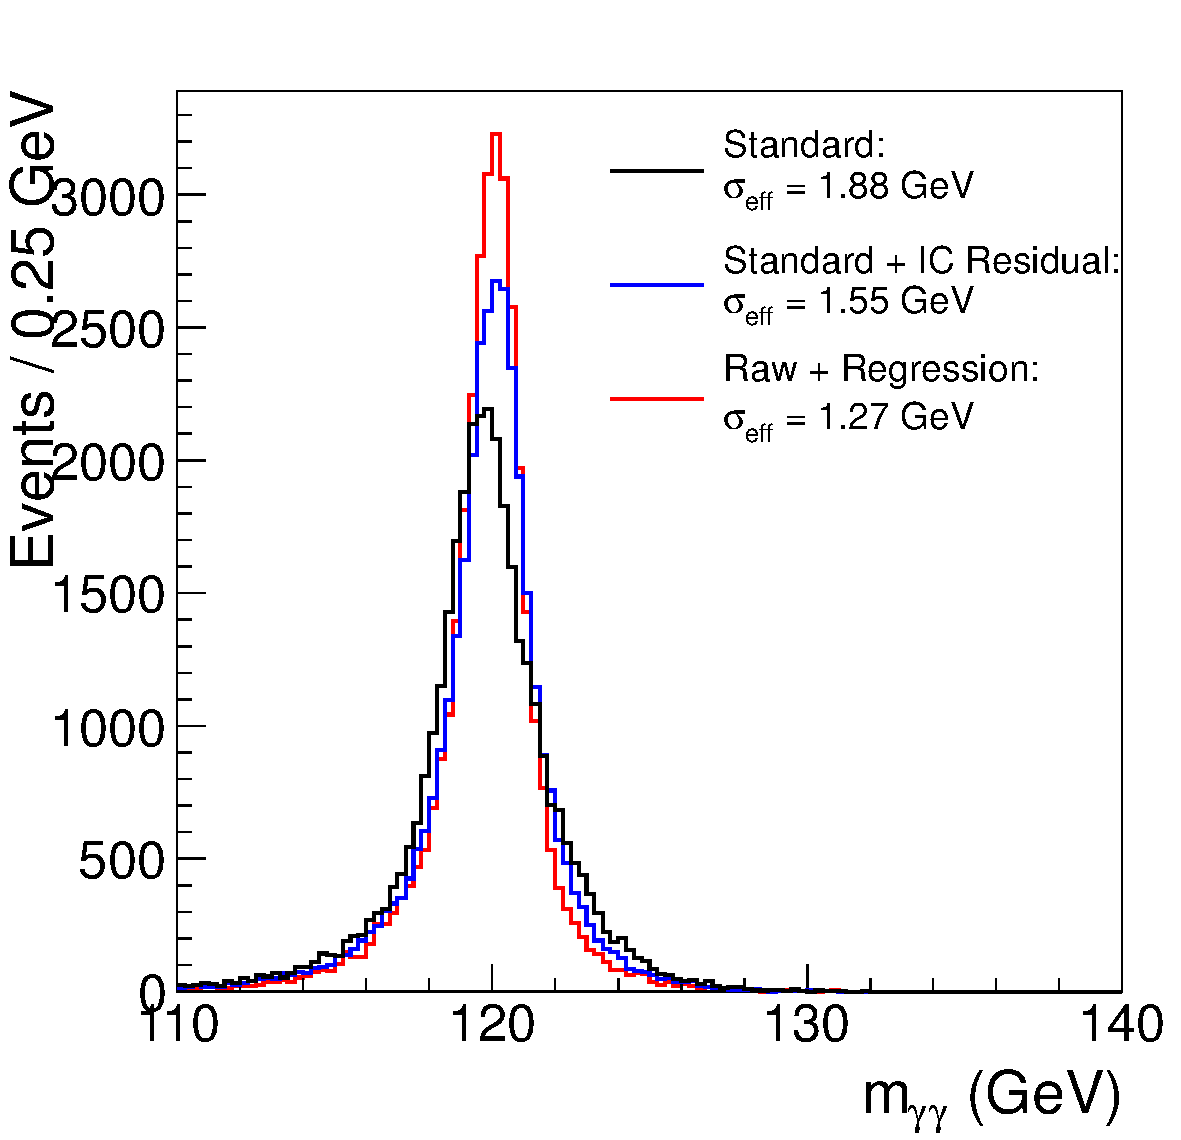
\includegraphics[width=.6\textwidth]{hgg7TeV/generalPlots/regrresall.pdf}
\label{fig:mcregrcomparison}
\caption{Comparison of the diphoton mass peak in MC Higgs with a mass of 120 GeV using different 
measurements of the photon energy. The black line 
is from using the raw energy of the supercluster, the blue is from using the analytic fit method 
and the red from using the regresssion method. The quantity $\sigma_{eff}$,
the narrowest range in $\mgg$ which contains 68\% of the distribution, is given for each peak.}
\end{center}
\end{figure}

An estimate of the per-photon energy resolution, $\sigma_{E}$, is obtained by training a second 
regression BDT targetting the the absolute deviation between the correction estimated by the 
first BDT and the true correction to generator level. This second BDT is trained on an independant
set of events to the first. The per-photon resolution is used to calculated an estimate of the 
per-event mass resolution, $\sigma_{\mgg}$, which is used during the event selection 
(Section~\ref{sec:eventselection}). An additional regression BDT is trained on $Zee$ MC which is used
to compare the supercluster energy scale in data and MC.

\subsubsection{Energy Scale Measured in Data}
Despite correcting the energy of the photons using the regression technique, discrepancies between data and
MC are still observed. This is due to additional detector effects which may not be simulated, such as the
time dependance of the ECAL crystal transparency. Further corrections are
derived based on $\Zee$ data which provides an invariant mass peak with almost no background constructed from 
electromagnetic objects which are reconstructed using a similar procedure to photons.
The energy scale of the superclusters is measured by matching the electron
invariant mass peak in data to that in MC. This is acheived using an analytic fit to the $\Zee$ peak in data and MC
separately. The natrual peak of the $Z$ is described using a Breit-Wigner distribution whose parameters are fixed
to those given by the Particle Data Group (PDG REF), $m_{Z}=91.188,~\Gamma_{Z} = 2.495$. This is then convoluted 
with a Crystal Ball (CB) which describes the resolution effects of the calorimeter and energy losses from 
bremsstrahlung before the ECAL. The CB parameters, $\Delta m$ \ldots, are the free parameters of the fit.

The values of these fitted parameters varies with the potition of the supercluster ($|\eta|$). Moreover the
variation in data is strongly dependant on the run during which the data were taken. The scale is extracted in 
six run ranges and four $|\eta|$ regions to account for this effect. 
The difference between MC and data with time is less dependant on whether the electron showered or not which 
is characterised by the $\rnine$ of the supercluster. The data-MC difference in each $|\eta|$ region is measured
a second time after applying the first set of corrections to the data and obtaining the residual difference
for electrons with $\rnine<0.94$ and $\rnine>0.94$ separately. The final energy scale correction is then defined
as the product of the two corrections. The relative correction, 

\begin{equation}
1-\Delta P = 1 - \frac {\displaystyle \Delta m_{data} - \Delta m_{MC} }{\displaystyle m_{Z} }
\end{equation}

is applied to the photons in data. The values for the scale in each category are given in 
Table~\ref{tab:scalecorr}. The uncertainties on these measurements are primarily due to 
the difference in the $\rnine$ distribution of electrons and photons. In addition, smaller systemaitcs
are included due to the variation of the measurements when changin the electron selection and
between using the electron-trained and photon-trained regression corrections.
These uncertainties are incorperated into the signal model for the purposes of 
signal extraction as described in Section~\ref{sec:signalmodel}.

\subsection{Vertex Selection}
\label{sec:vertexselection}

\subsection{Photon Identification}
\label{sec:photonidentification}

A large portion of the fake background in the $\Hgg$ search is due to high momentum neutral mesons
which decay to two photons where both the photons are combined into the same supercluster. 
Information from the shower shape of the photon supercluster can be used, as well as the 
energy isolation within the calorimeter, in order to distinguish these from real photons
from the primary interaction point. A BDT was trained on MC samples to combine the relavant information
into a single photon identification (ID). The signal used for the training was taken from Higgs decaying to
two photons MC with mass 121 GeV while the background was taken from non-prompt photons in the Gamma+Jet sample.
Before training, events are required to pass a loose preselection designed to avoid training 
where the MC is unable to properly describe the data and to match the variables used in the trigger.
In addition, photon candidates are removed if there is a reconstructed GsfElectron matched to the 
photon supercluster with no matching conversion reconstruction. This greatly reduces the contribution
from $\Zee$ faking photons. The same preselection is applied to all MC and data for extracting the signal.
The efficiency of the preselection for signal was measured in $\Zee$ data and MC using a tag-and-probe 
method (REF). The results are shown in Table~\ref{tab:sigeffpresel}. 

\begin{table}
\begin{center}
\begin{tabular}{| l | c | c | c |}
\hline
\textbf{Category} & \textbf{Data} & \textbf{MC} & \textbf{Data/MC} \\
\hline
EB $\rnine>0.9$ & 0.9267 $\pm$ 0.0012 & 0.9275 $\pm$ 0.0006 &0.999 $\pm$ 0.0013 \\
EB $\rnine<0.9$ & 0.8882 $\pm$ 0.0023 & 0.9025 $\pm$ 0.0010 &0.984 $\pm$ 0.0025 \\
EE $\rnine>0.9$ & 0.9442 $\pm$ 0.0010 & 0.9387 $\pm$ 0.0009 &1.006 $\pm$ 0.0014 \\
EE $\rnine<0.9$ & 0.8639 $\pm$ 0.0010 & 0.8517 $\pm$ 0.0011 &1.014 $\pm$ 0.0015 \\
\hline
\end{tabular}
\label{tab:sigeffpresel}
\caption{Signal efficiency for the preselection measured in data and MC using tag-and-probe in
$\Zee$ events. The ratio Data/MC are applied as corrections to the signal MC for the purposes
of signal modelling. The uncertainties listed here are statistical only.}
\end{center}
\end{table}


The input variables are chosen to be insensitive to the kinematics of the diphoton system itself
including the diphoton invariant mass. The first set of variables describe the shower shape of the 
supercluster: $\hoe$, $\sigieie$, $\rnine$ and the energy weighted widths of the supercluster in
$\eta$ and $\phi$ ($\sigma_{\eta},~\sigma_{\phi}$). The $\eta$ of the supercluster is 
included as the shower shape is dependant on the position within the calorimeter. 
The second set of input variables describe the
isolation of the photon in the calorimeter and tracker scaled to account for 
the additional expected energy density due to pileup, $\rho$. These are the sum of the track isolation, 
calculated relative to the chosen vertex and the vertex giving the maximum track isolation,
ECAL isolation and HCAL isolation in a cone with $\Delta R<0.3$ minus $\rho$ times the effective area 0.17
and the absolute ECAL and HCAL isolations within cones of $\Delta R <0.3$ and $\Delta R<0.4$ 
respectively. In addition, the number of reconstructed vertices in the bunch crossing is included
to reduce the pileup dependance of the isolation variables. 

A separate BDT is trained for application in the ECAL barrel and endcaps as the shower
shape and isolation variables are rather distinct between the two components. 
A cut is made on the photon ID BDT output to select events used for the signal extraction which
keeps practically all ($>99\%$) of the signal while removing around 22\% of background events.
The cut is choson to be loose as the output of the photon ID will be used as input for the 
event selection (diphoton BDT) desribed in Section~\ref{sec:diphotonbdt}, 

\section{Event Selection}
\label{sec:eventselection}

In addition to passing the preselection, the two photons are required to pass mass-dependant transverse 
momenta cuts, $p_{T}/\mgg > 1/3, 1/4$ for the leading and subleading $\pt$ photon respectively.
The final selection of diphoton candidates used for the signal extraction is based on using as much information 
in the event as possible to distinguish likely signal candidate events from the background. Although the 
photon ID BDT is successful at rejecting fake backgrounds, a large portion of the background is due to
real prompt photons from QCD processes. In order to distinguish these from a Higgs signal, 
the specific kinematics and toplogy of the event is exploited.


\subsection{Diphoton BDT}
\label{sec:diphotonbdt}
A BDT was trained to utilise the kinematics of the selected diphoton pair to discrimiate prompt photons
from QCD background from those produced by the decay $\Hgg$. These are the relative transverse momenta 
of the photons, $\pt^{1},~\pt^{2}$, their pseudo-rapidites, $\eta^{1},~\eta^{2}$ and the cosine of the 
angle between the two photons in the transverse plane $cos(\Delta\phi)=cos(\phi^{1}-\phi^{2})$.
In addition, information regarding the quality
of the objects, the two photons and the selected vertex, is included in the form of the output of the 
photon ID and the vertex probability. The per-photon resolution estimate, $\sigma_{E}$ is combined for
each photon to produce a per-event mass resolution estimate $\sigma_{\mgg}$ under the assumption that 
the correct vertex is chosen given by,

\begin{equation}
\sigma_{\mgg} (right-vtx) = \frac{\displaystyle 1}{\displaystyle 2} \mgg 
\sqrt{ \left( \frac{\displaystyle {\sigma_{E}^{1}}}{\displaystyle E^{1} } \right)^{2}
     + \left( \frac{\displaystyle {\sigma_{E}^{2}}}{\displaystyle E^{2} } \right)^{2}
     }
\end{equation}
where $E^{1},~E^{2}$ are the energies of the two photons.

Since the correct vertex is not always chosen, the mass resolution assuming the incorrect vertex is chosen
is calculated using the average beamspot length in data, $\sigma_{Z}=5.8cm$. In this case, the distance 
between the selected and true vertex will be distributed as a Gaussian with width $\sqrt{2}\sigma_{Z}$.
The contribution to the resolution, $\sigma_{\mgg}^{vtx}$ can be calculated analystically given the positions of
the two photons. The mass resolution estimator under the assumption that the incorrect vertex is chosen is 
given by the sum in quadrature of $\sigma_{\mgg}^{vtx}$ with the mass resolution assuming the correct vertex is chosen.
Both estimators for the mass resolution relative to the invariant mass, $\sigma_{\mgg}/\mgg~right/wrong-vtx$, 
are included as inputs to the diphoton BDT.




\begin{figure}[hbt!]
\begin{center}
  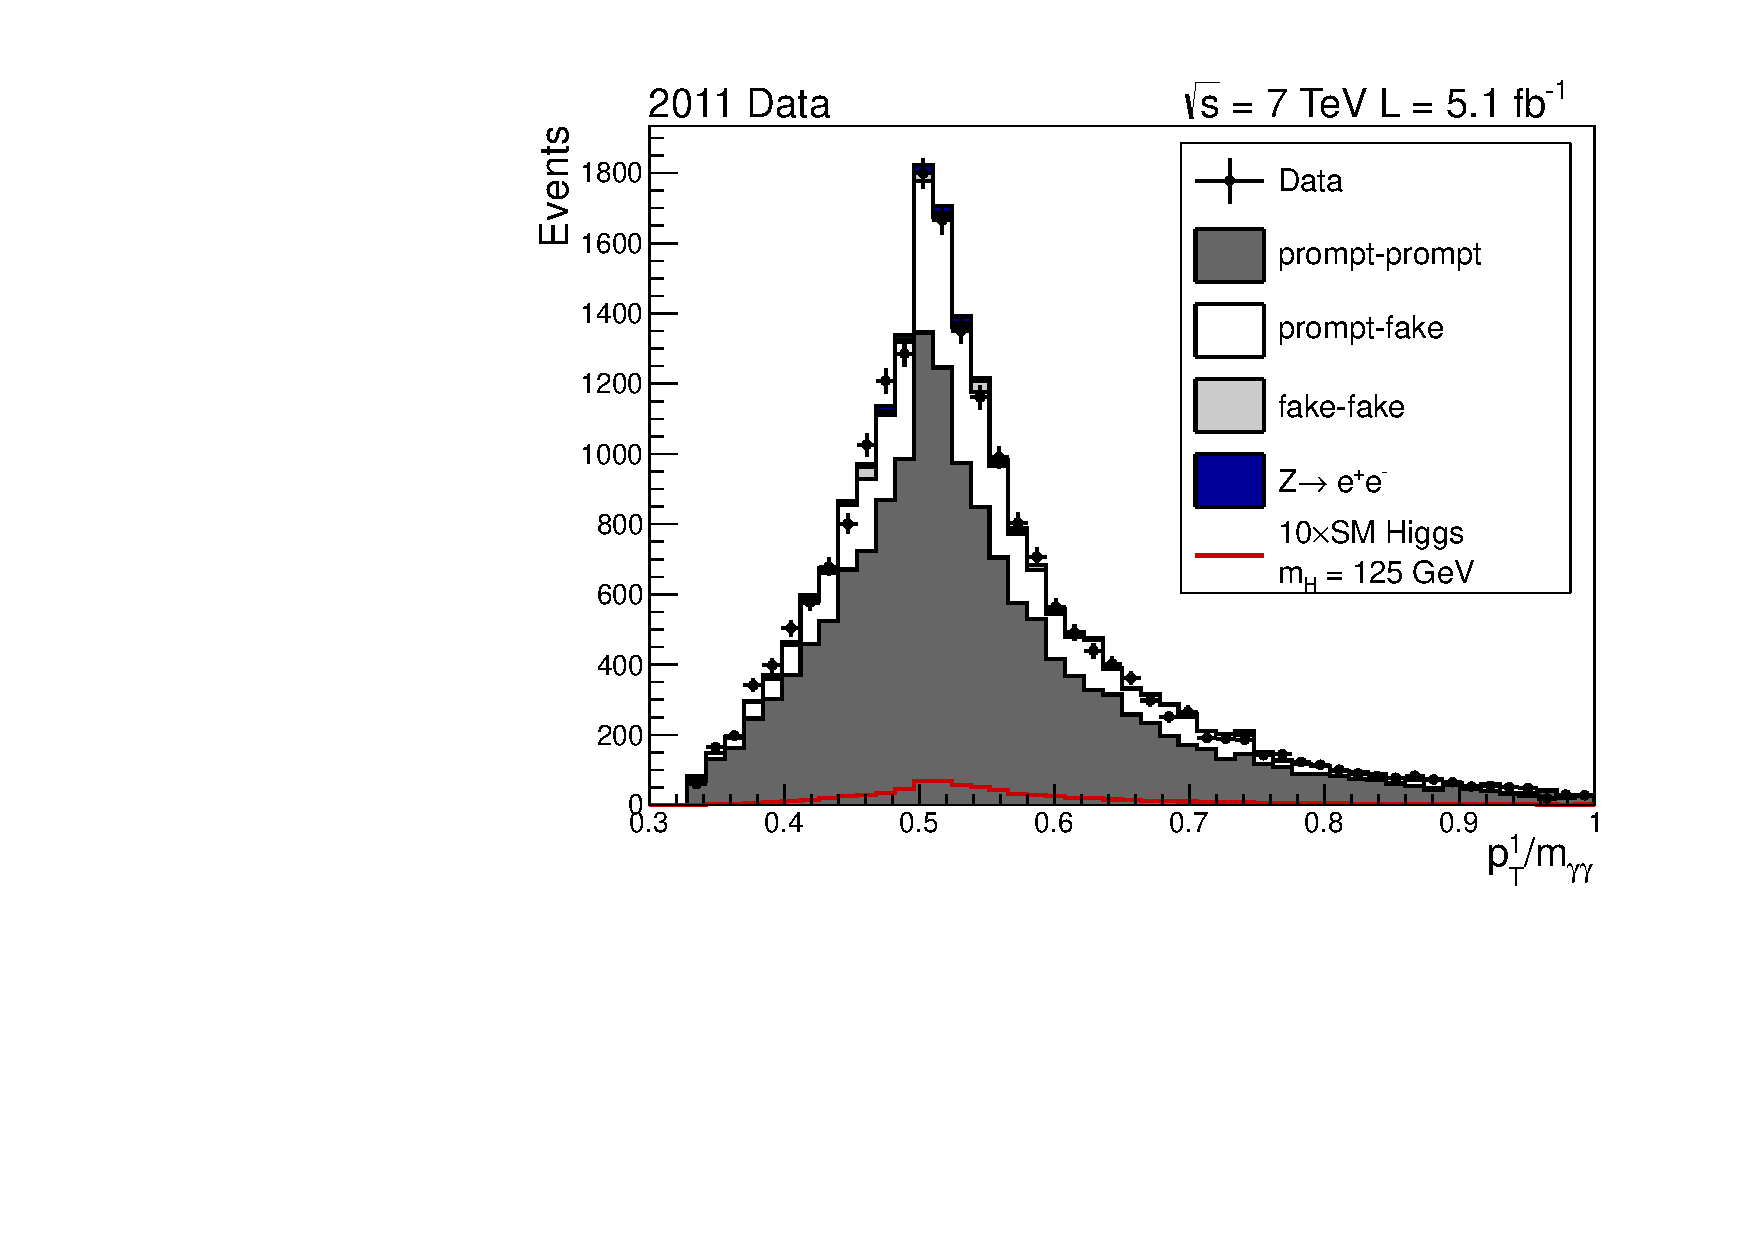
\includegraphics[width=0.48\textwidth]{hgg7TeV/variablePlots/pt_1om}
  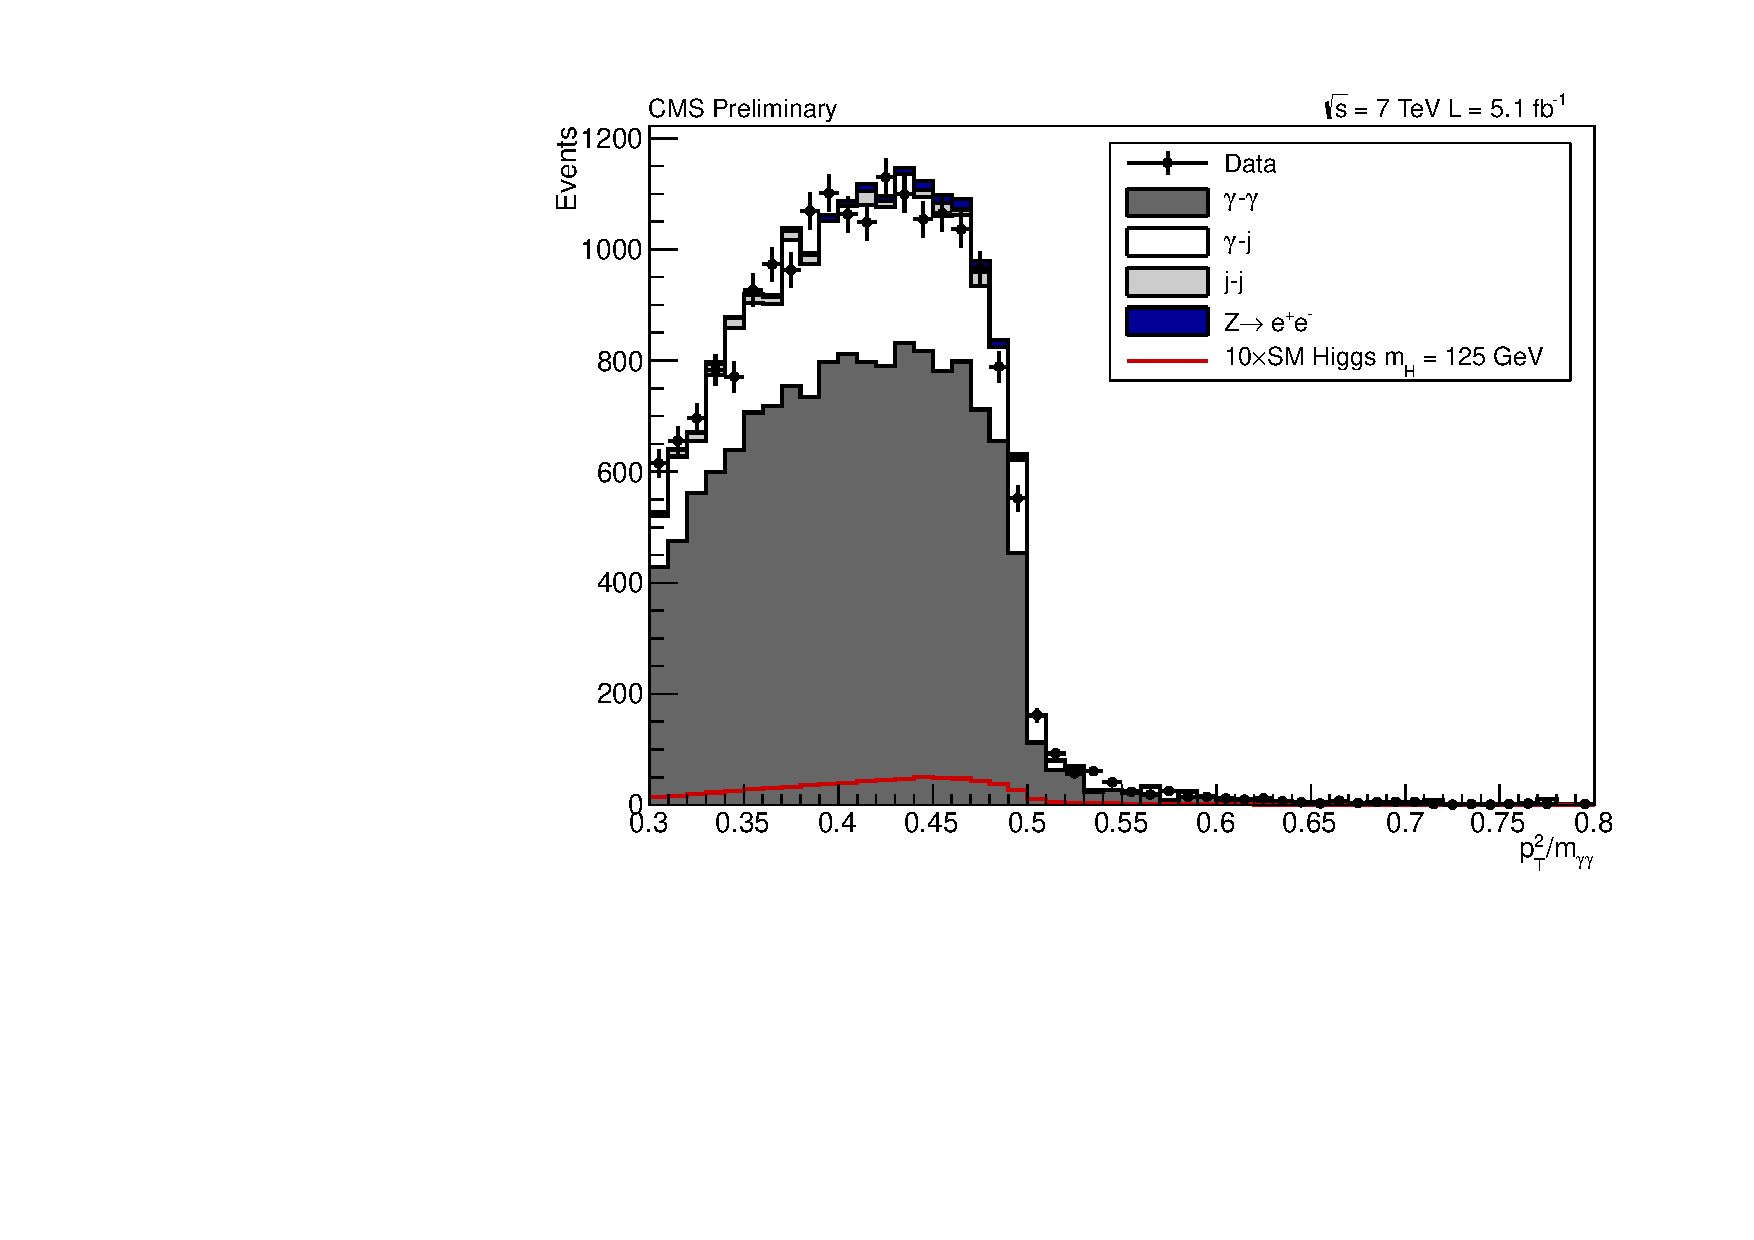
\includegraphics[width=0.48\textwidth]{hgg7TeV/variablePlots/pt_2om}\\
  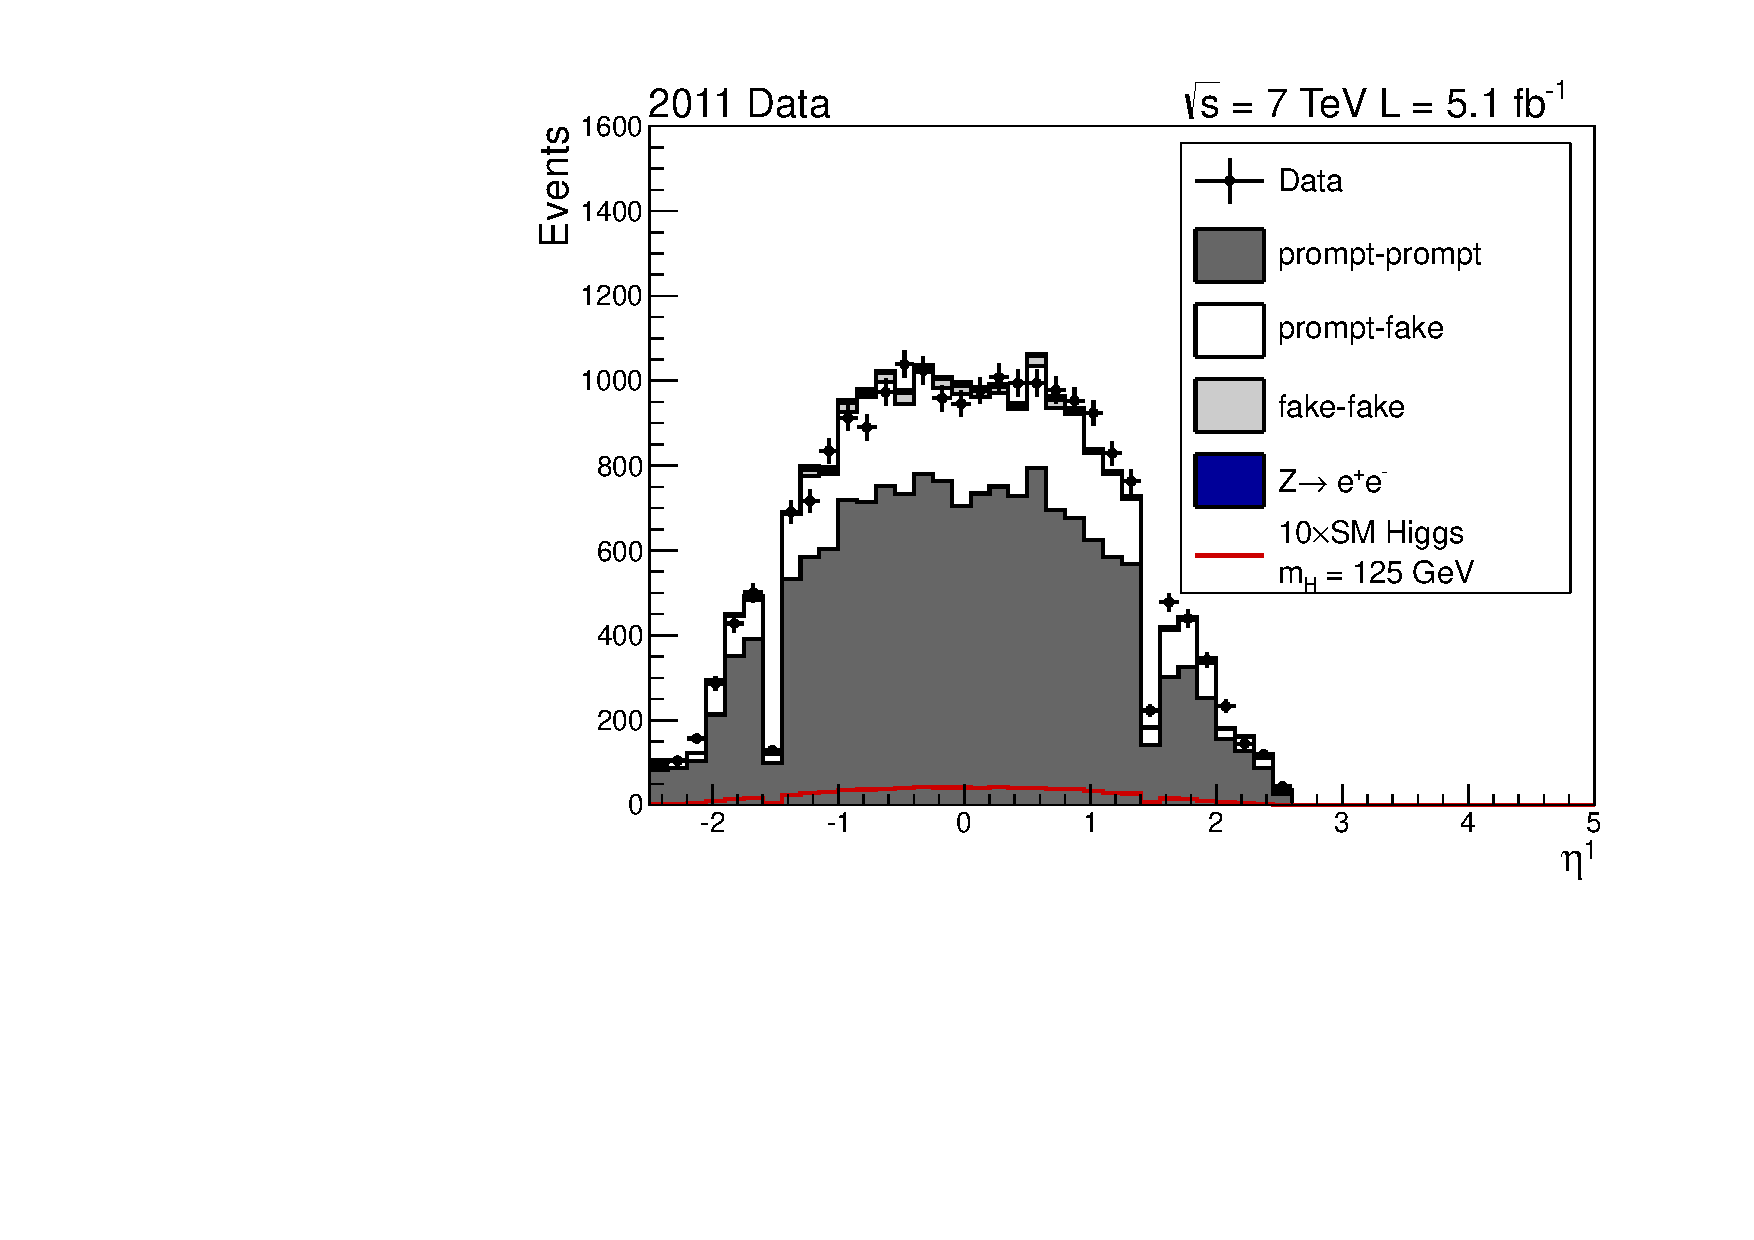
\includegraphics[width=0.48\textwidth]{hgg7TeV/variablePlots/phoeta_1}
  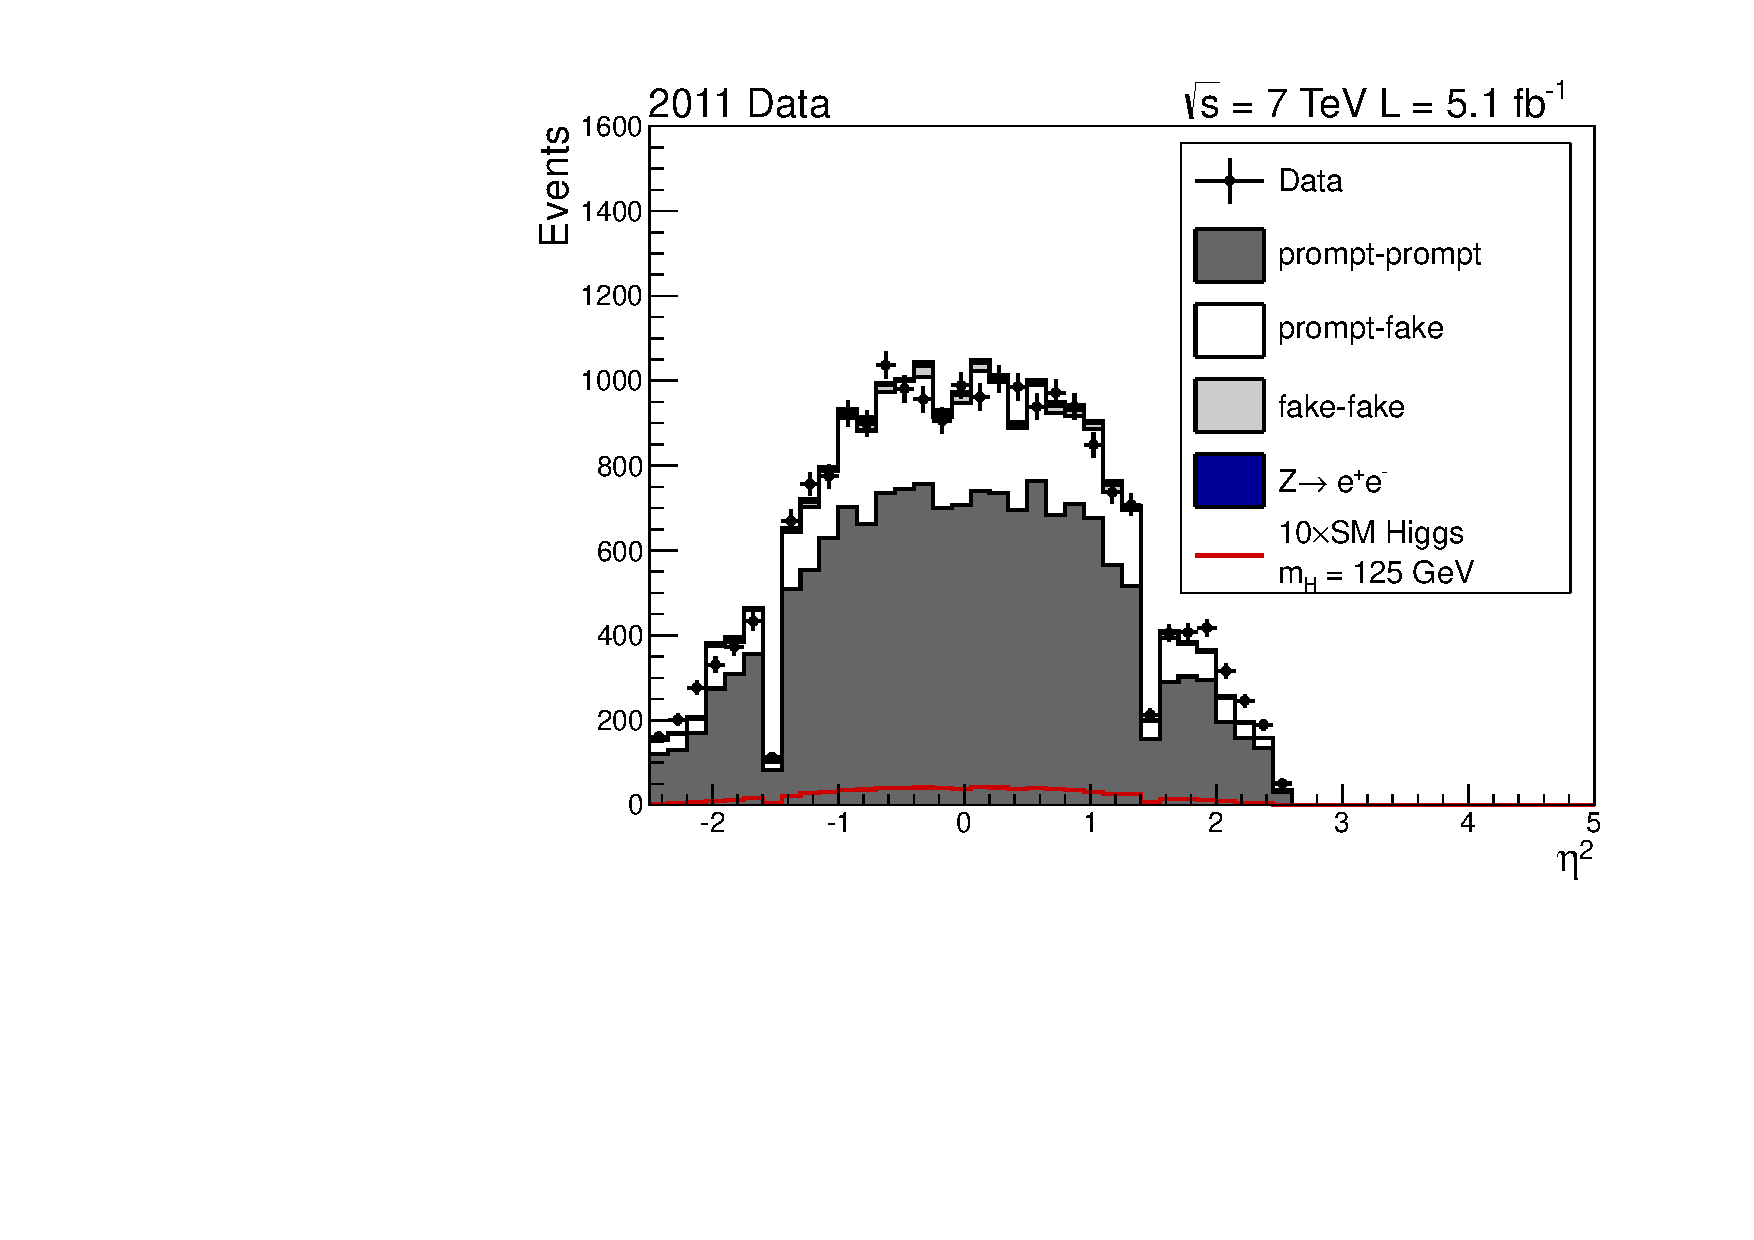
\includegraphics[width=0.48\textwidth]{hgg7TeV/variablePlots/phoeta_2}\\
  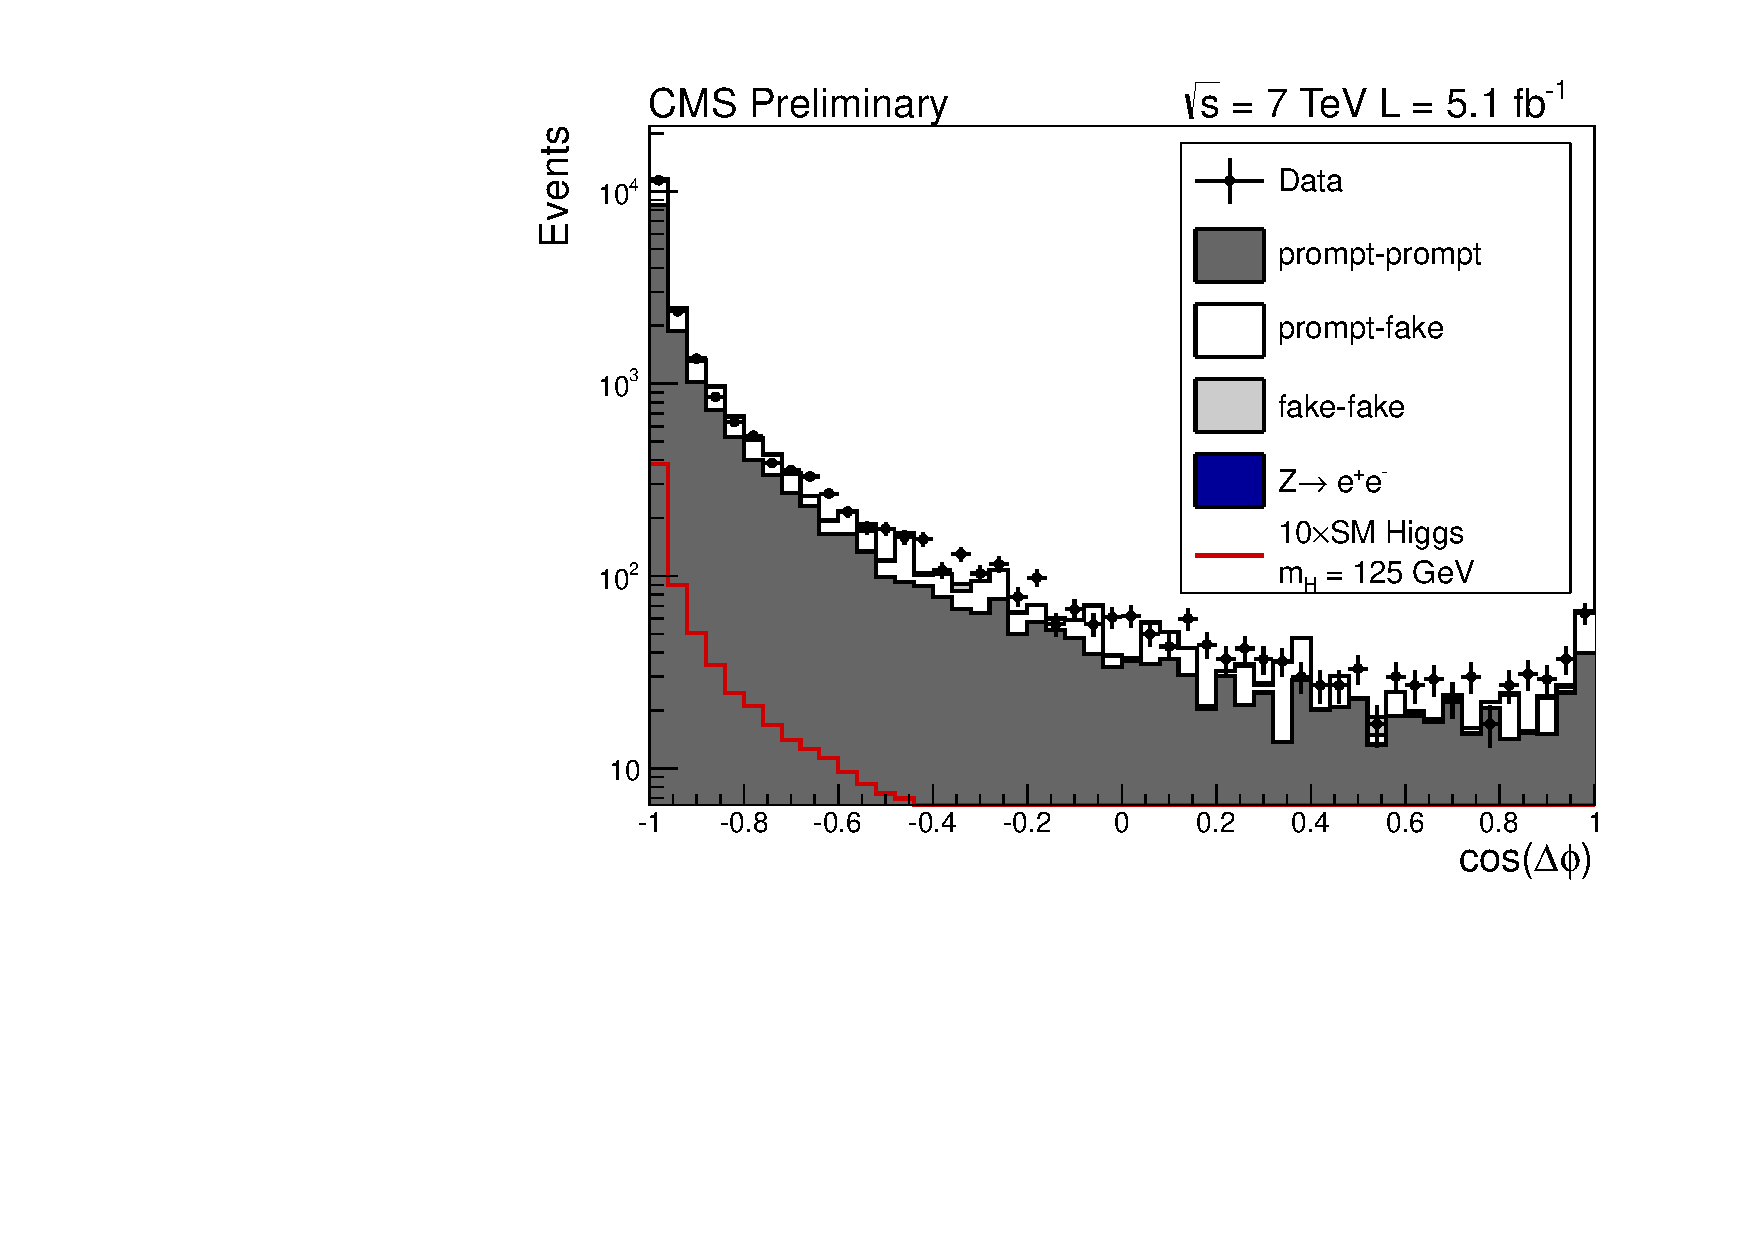
\includegraphics[width=0.48\textwidth]{hgg7TeV/variablePlots/cosdphi}
 \label{fig:diphotonbdtvars1}
 \caption{VARIABLES}
\end{center}
\end{figure}

\begin{figure}[hbt!]
\begin{center}
  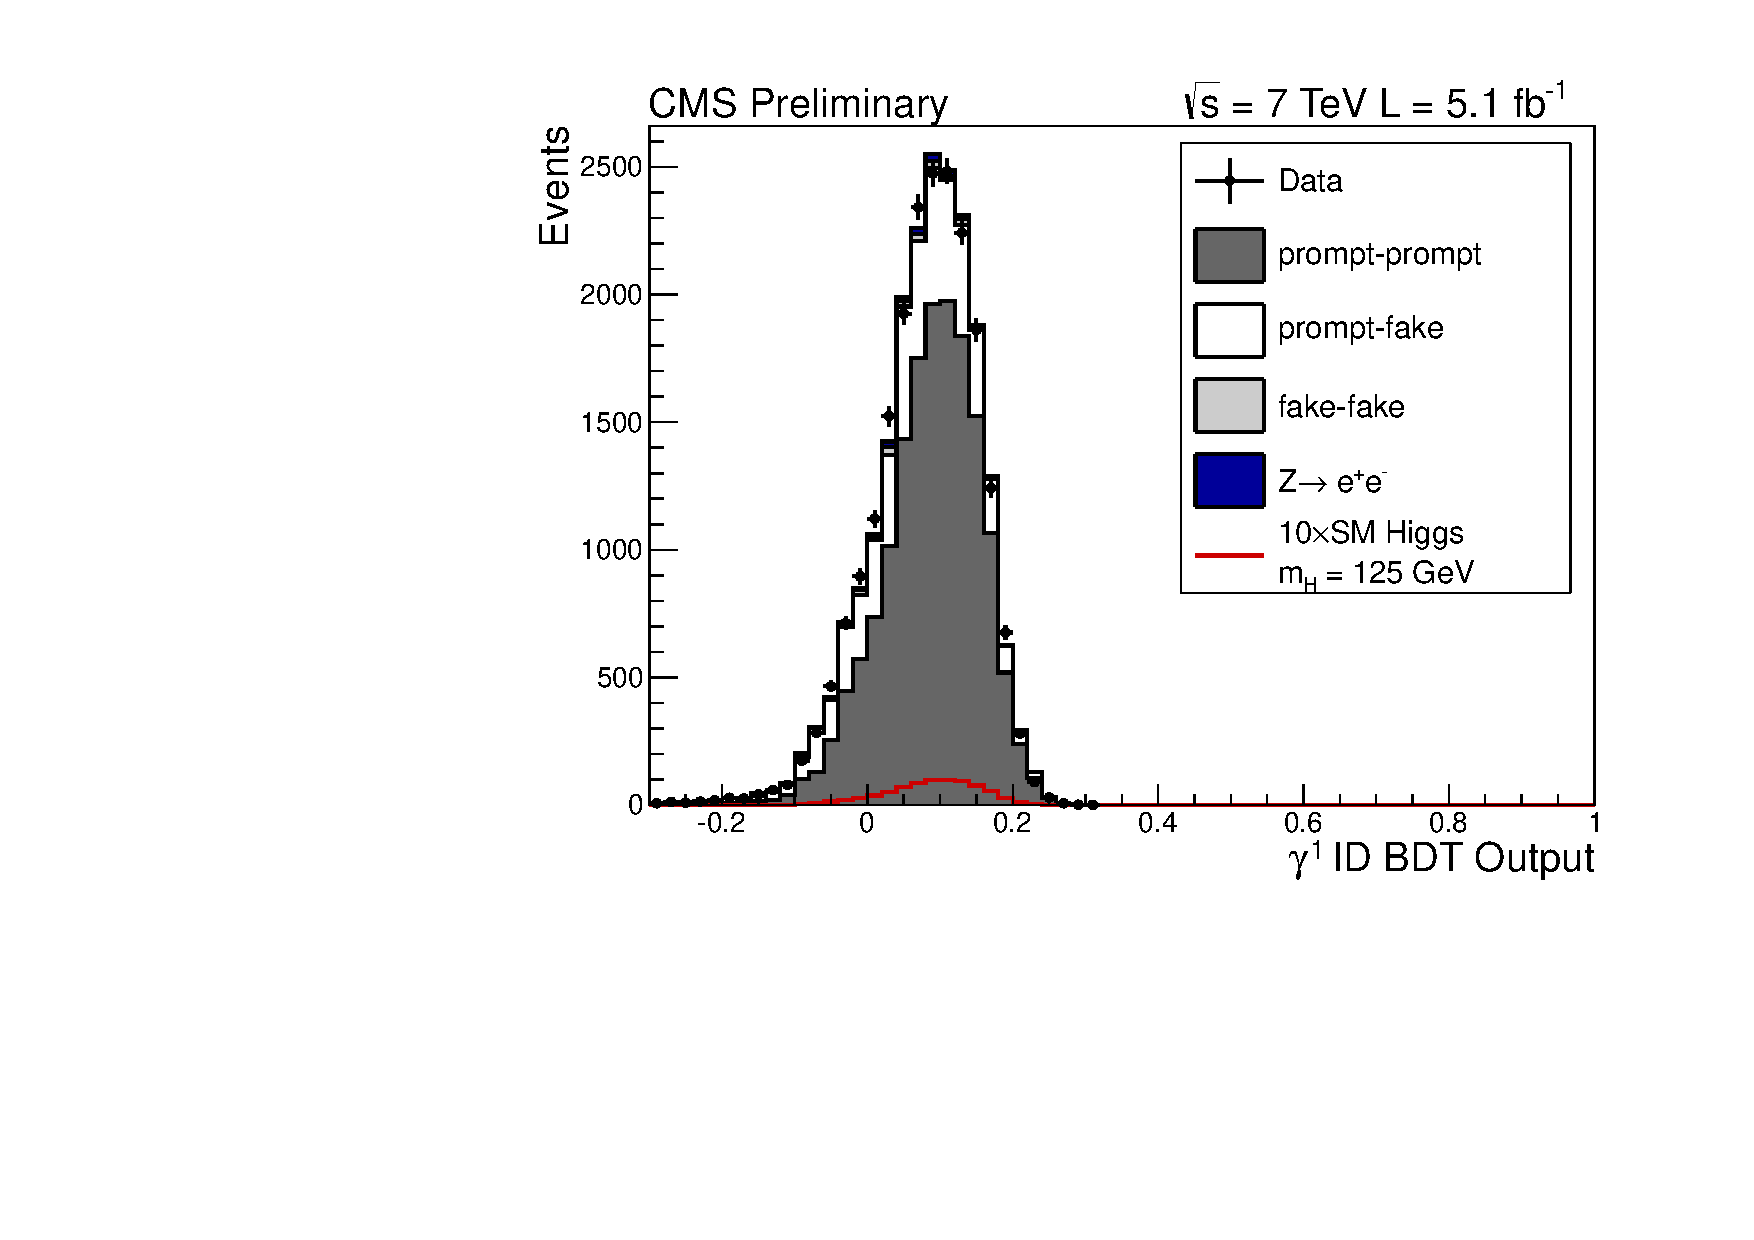
\includegraphics[width=0.48\textwidth]{hgg7TeV/variablePlots/phoid_1}
  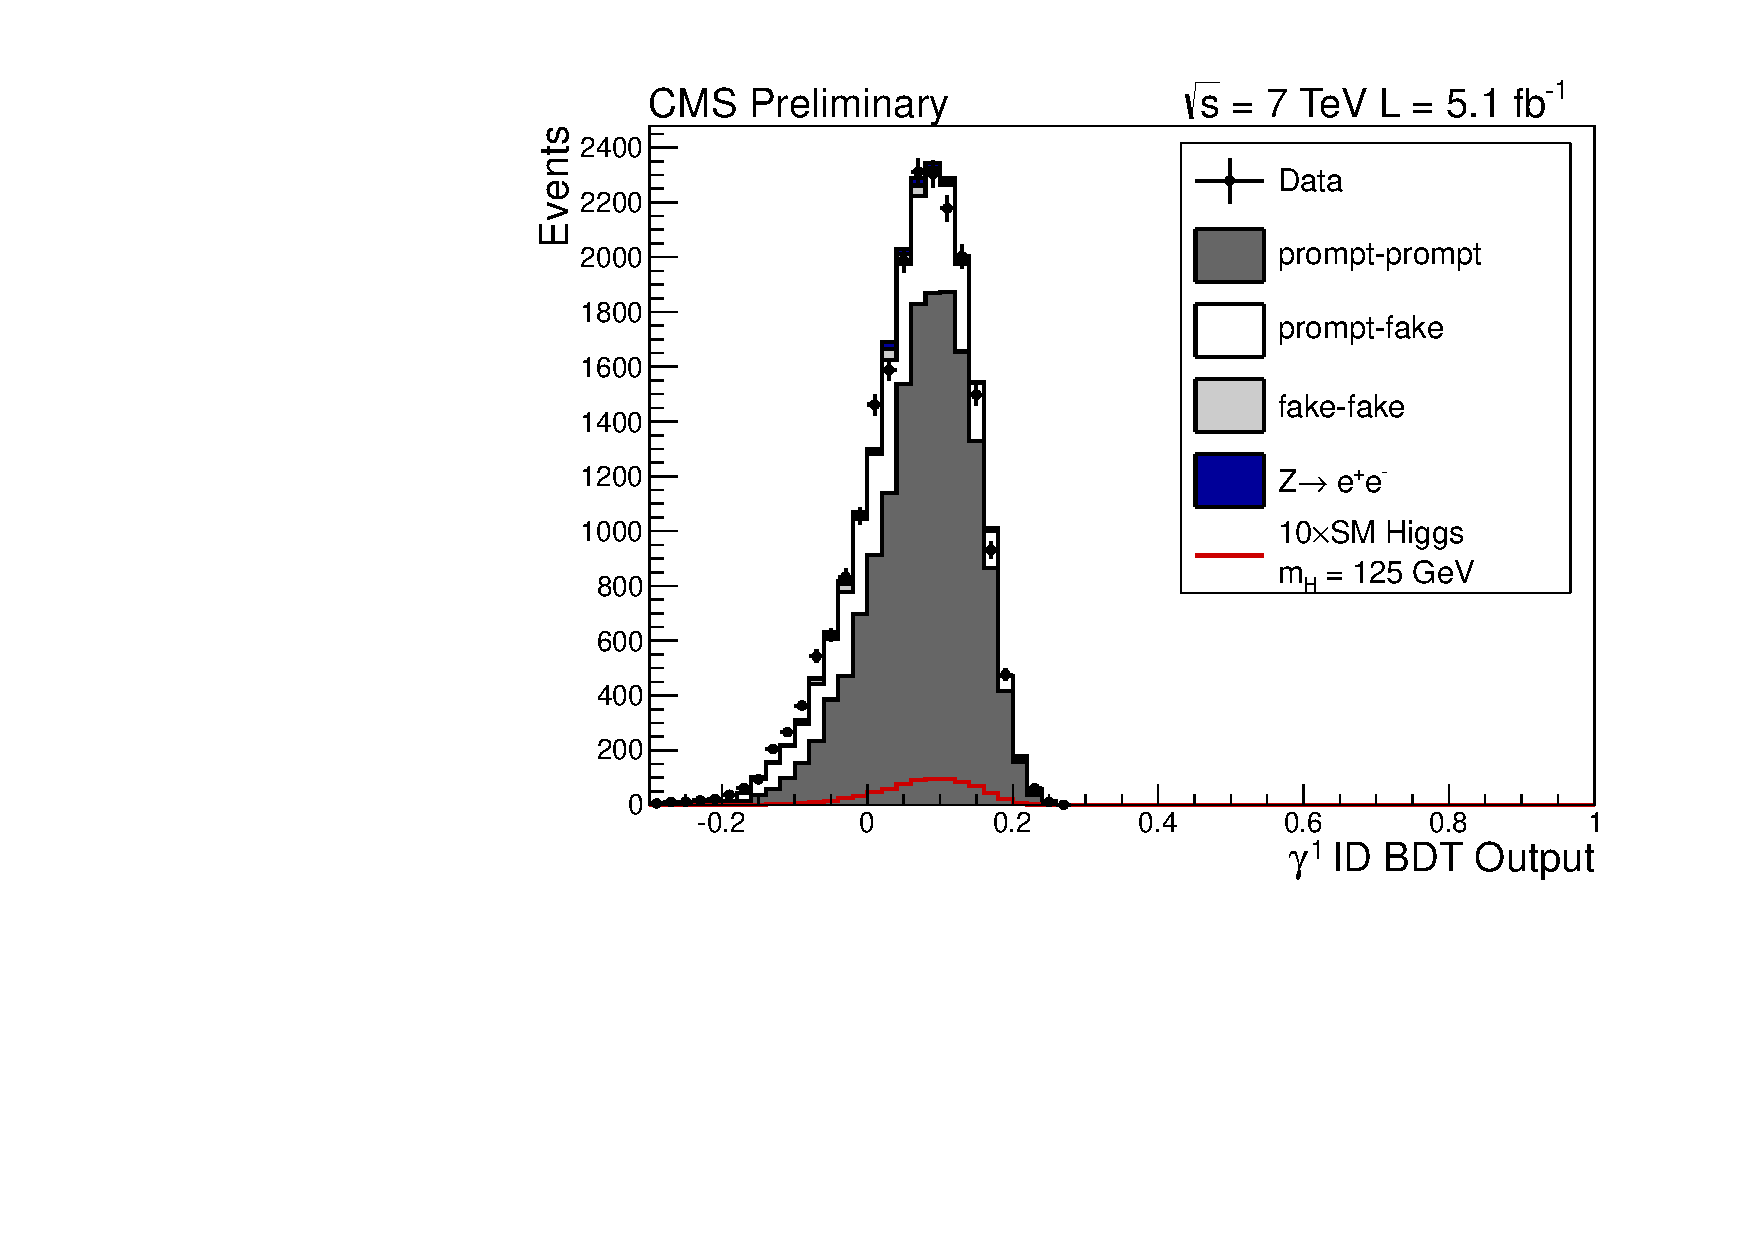
\includegraphics[width=0.48\textwidth]{hgg7TeV/variablePlots/phoid_2}\\
  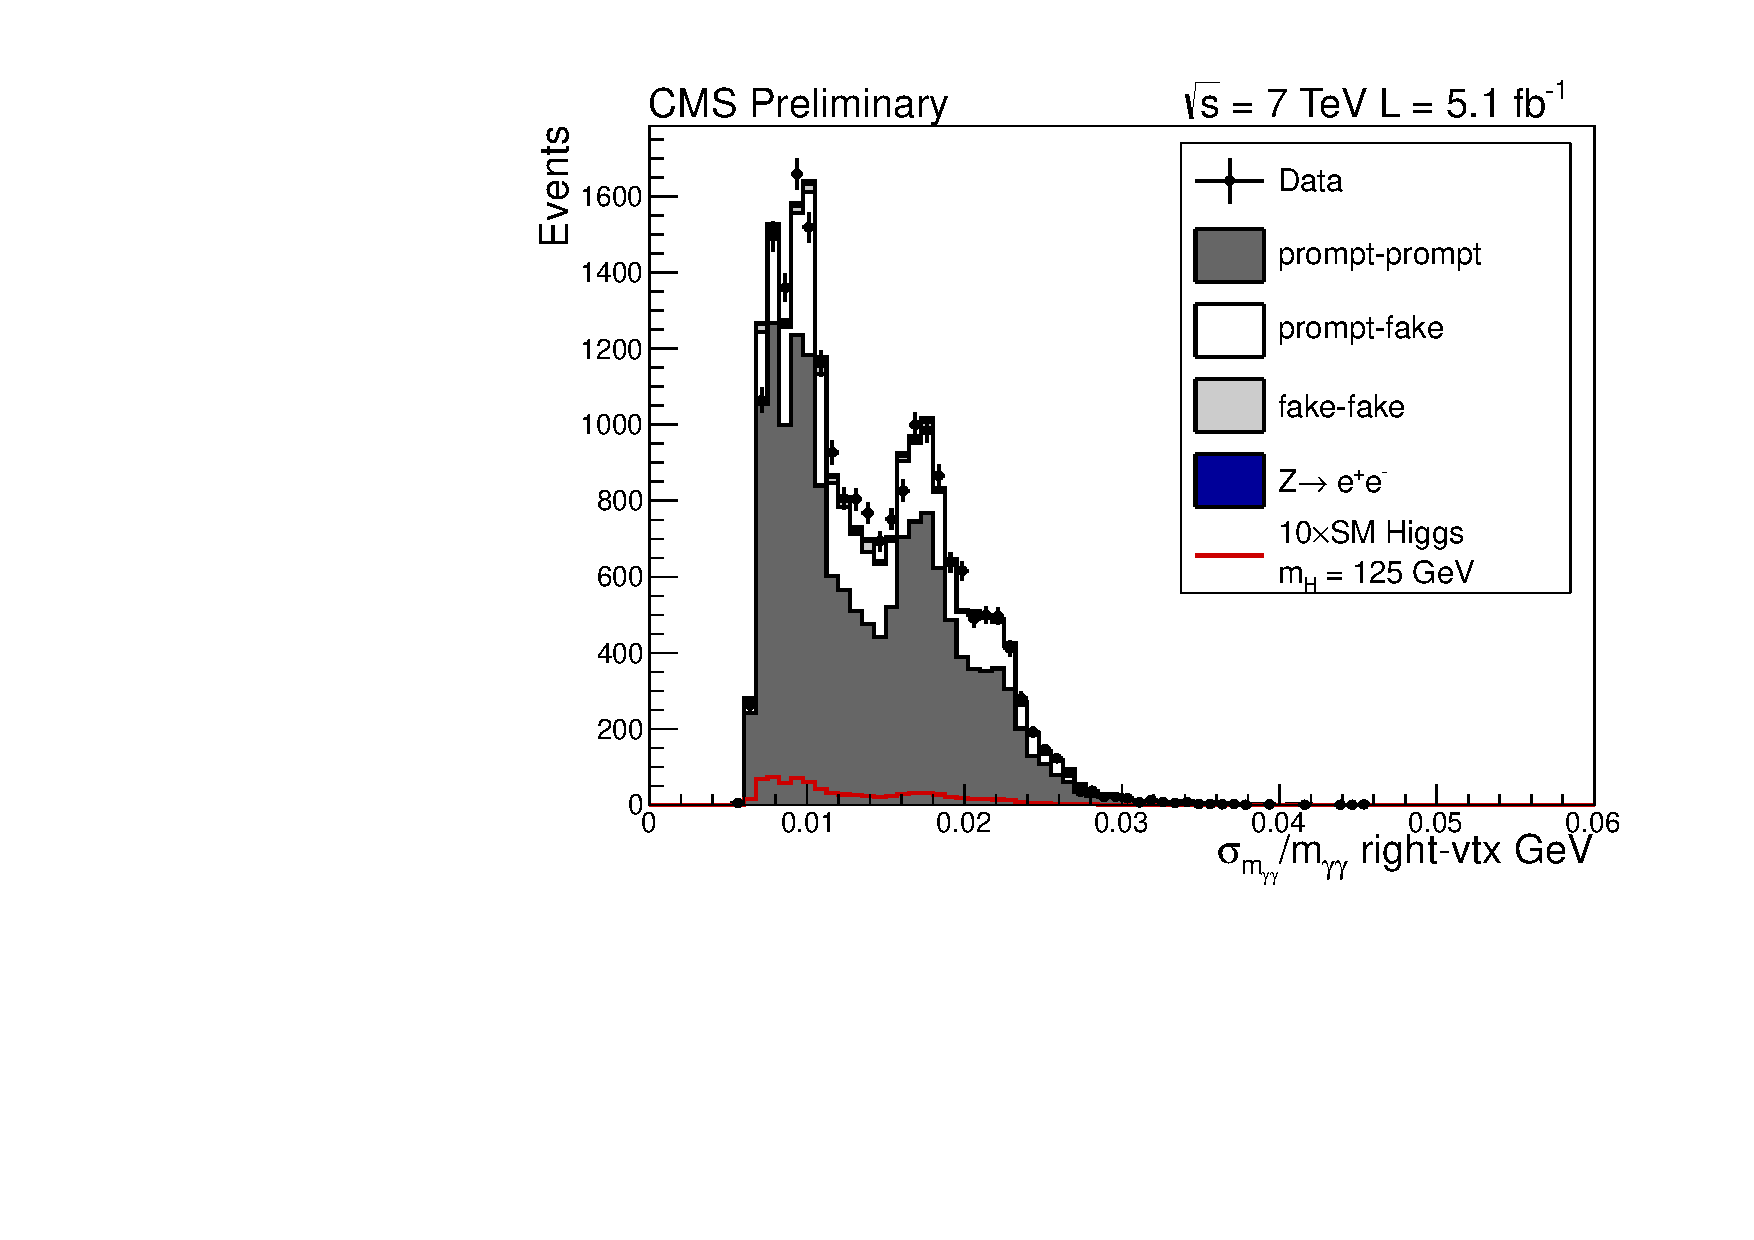
\includegraphics[width=0.48\textwidth]{hgg7TeV/variablePlots/sigmrv}
  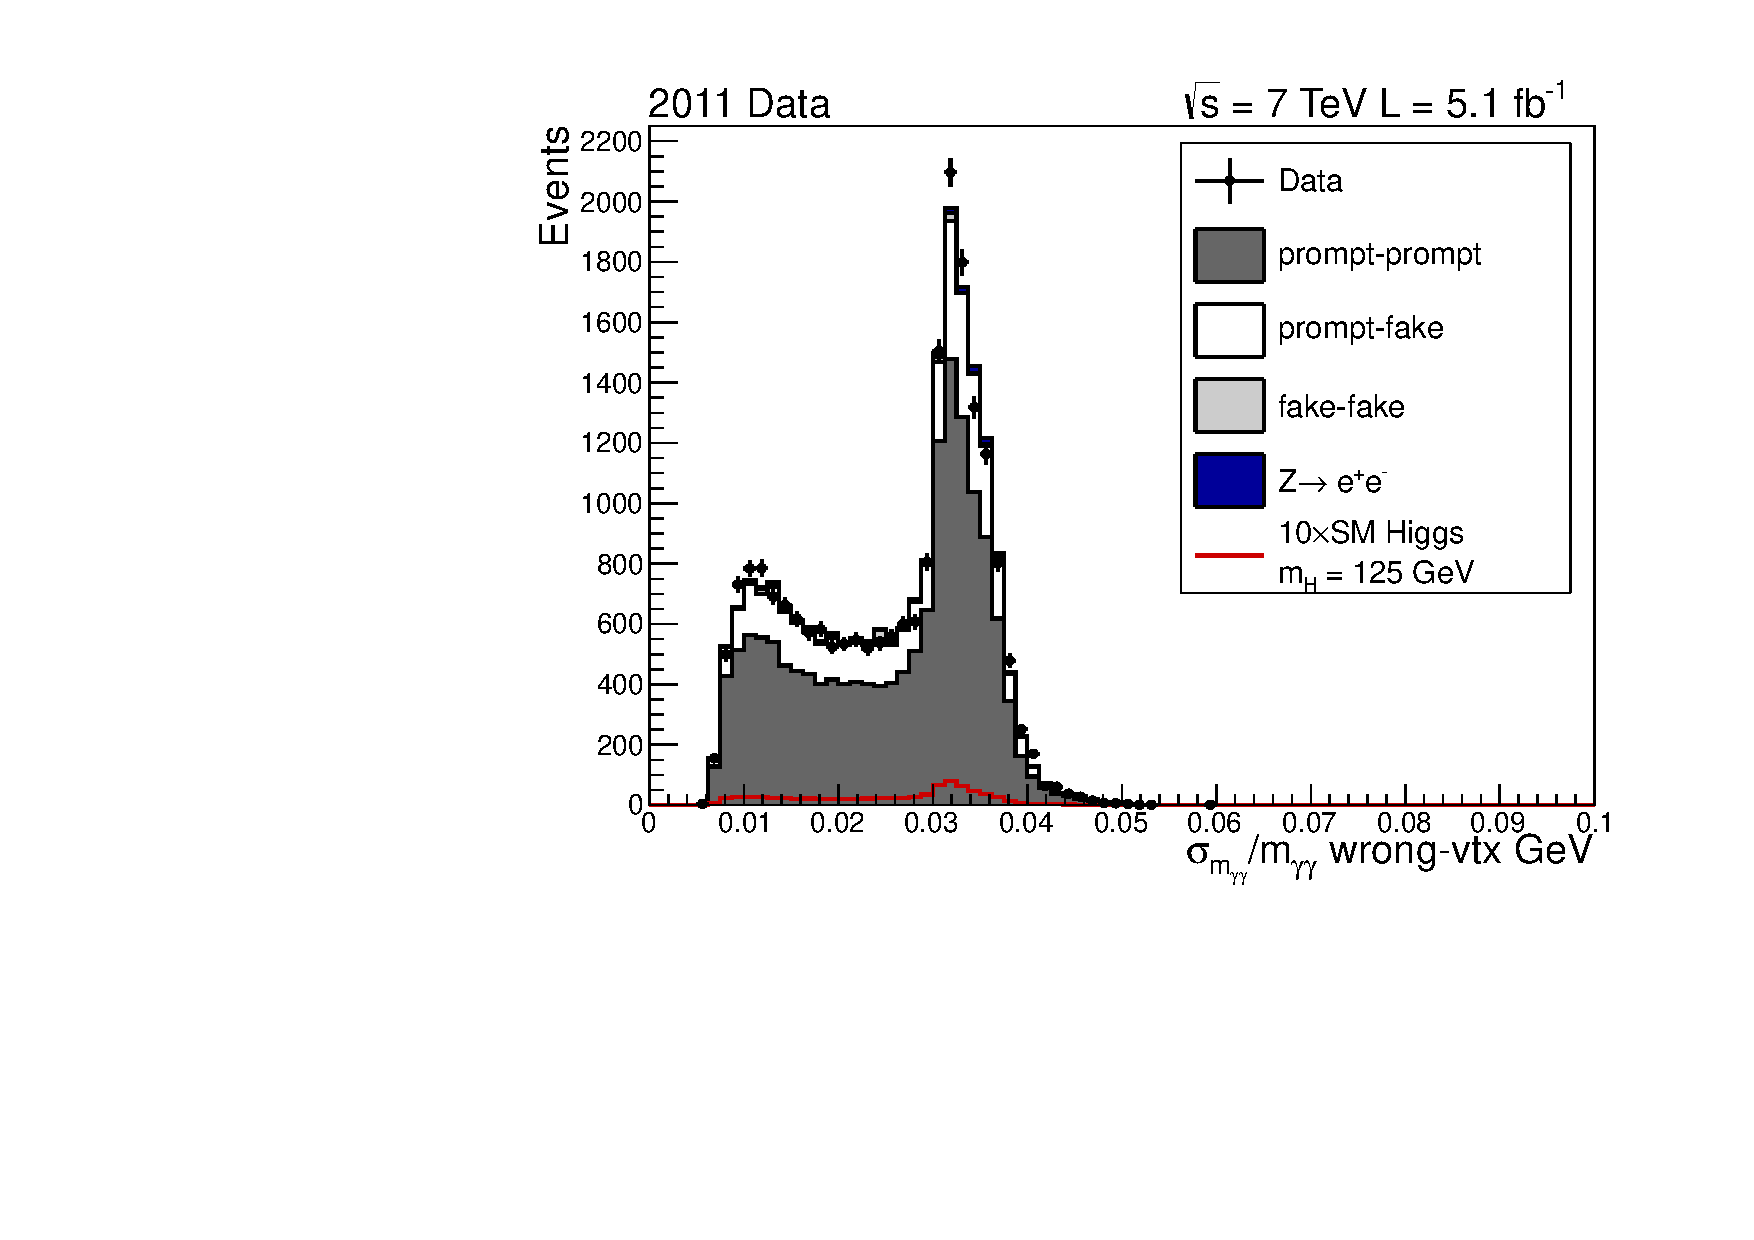
\includegraphics[width=0.48\textwidth]{hgg7TeV/variablePlots/sigmwv}
 \label{fig:diphotonbdtvars2}
 \caption{VARIABLES}
\end{center}
\end{figure}

Figure~\ref{fig:massmcdata} shows the invariant mass distribution in data and MC for events passing the full
selection with a diphoton BDT output greater than 0.05.

\begin{figure}[hbt!]
\begin{center}
  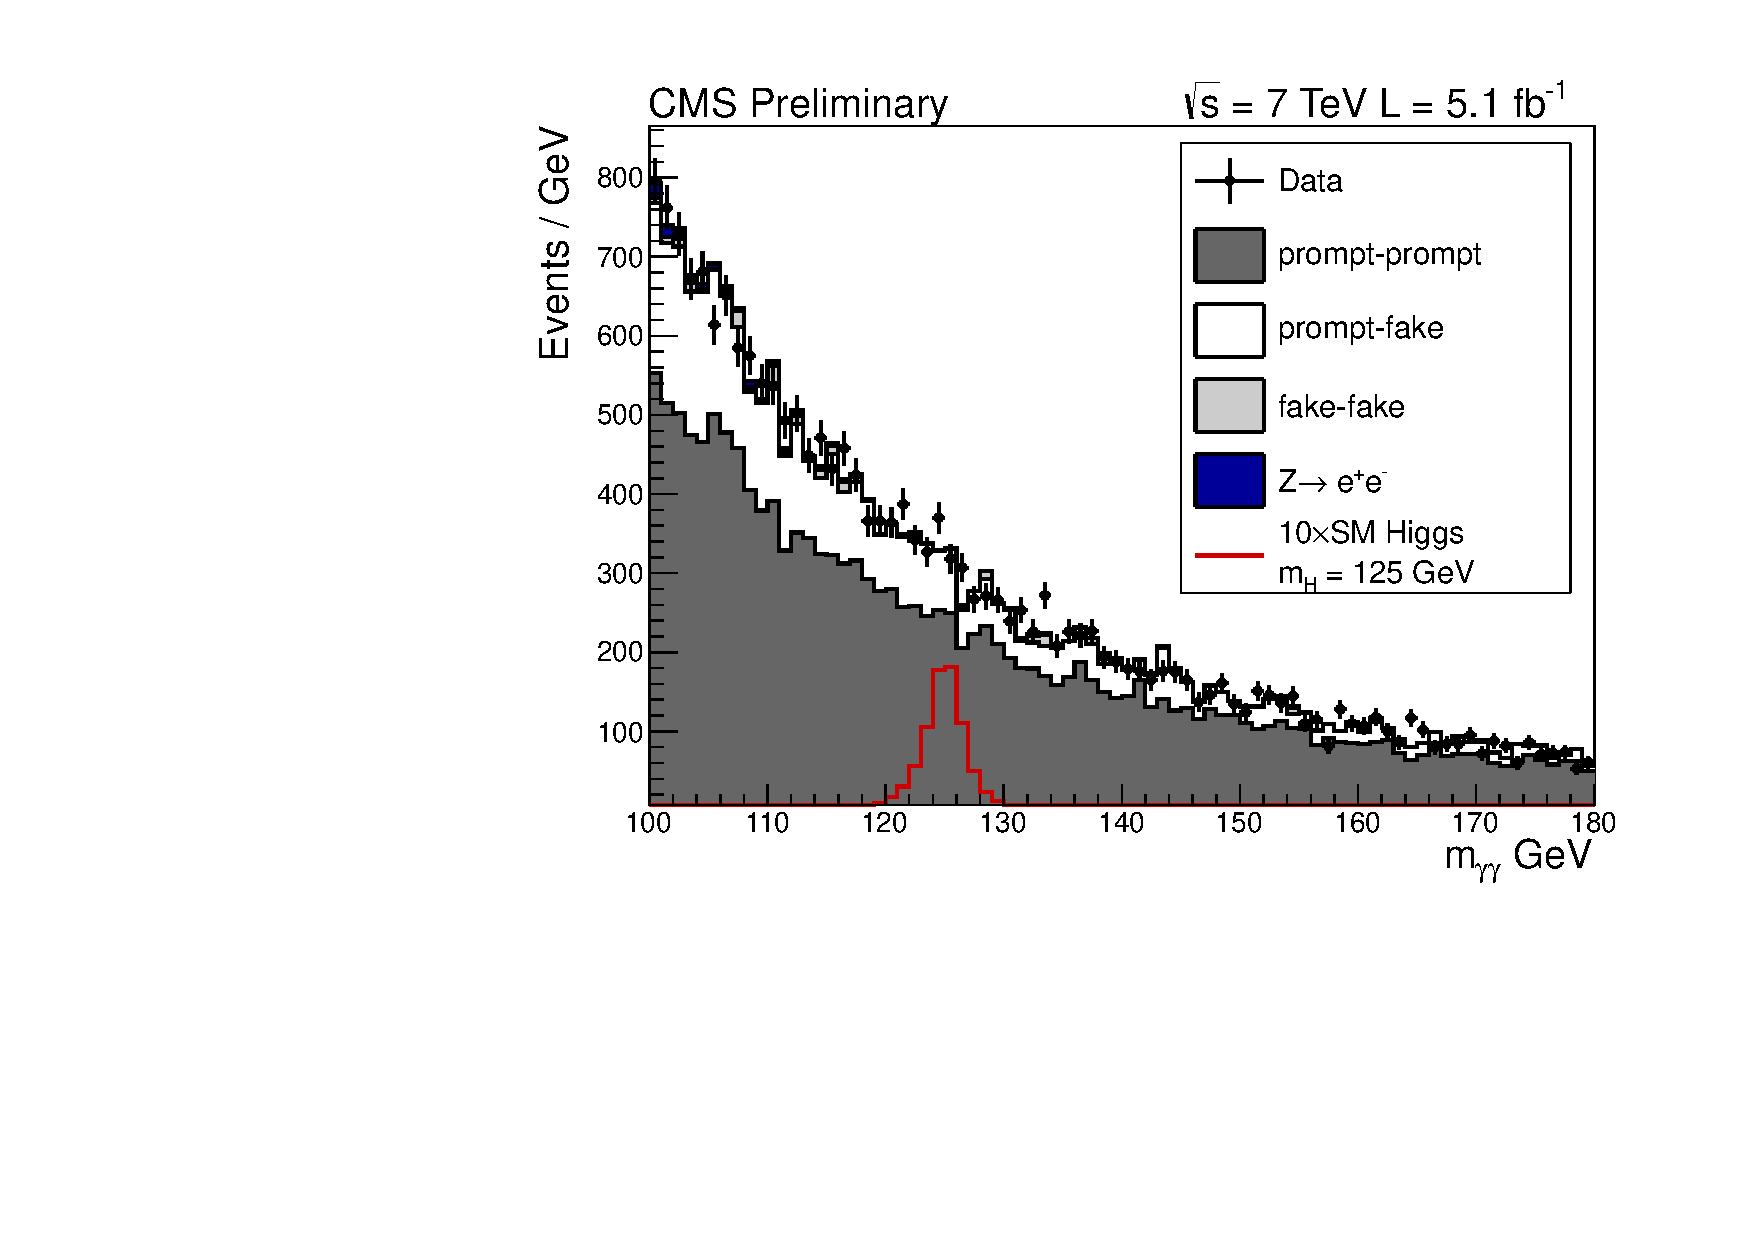
\includegraphics[width=0.5\textwidth]{hgg7TeV/variablePlots/mass}
 \caption{Invariant mass distrobution in data and MC after applying the full event selection in the
 range 100 to 180 GeV. The contribution expected from a SM Higgs with mass 125 GeV, scaled by 10, 
 is shown in red. }
 \label{fig:massmcdata}
\end{center}
\end{figure}

\subsubsection{Diphoton BDT Validation with $Zee$}

\subsection{Dijet Tagging}



